\fancyhead[C]{Section 16.4}
	\fancyhead[R]{\daytwentyfour}

\iftoggle{questions}{
\begin{center}{\large \textbf{Math 2551 Worksheet: Curl, Divergence, Green's Theorem}}
\end{center}


\begin{enumerate}
	
	\item Below is a plot of a vector field $\bF(x,y)$.  Use this to decide whether the values of $\curl \bF \cdot \bk$ and $\Div \bF$ in each quadrant are positive, negative, or zero.
	
	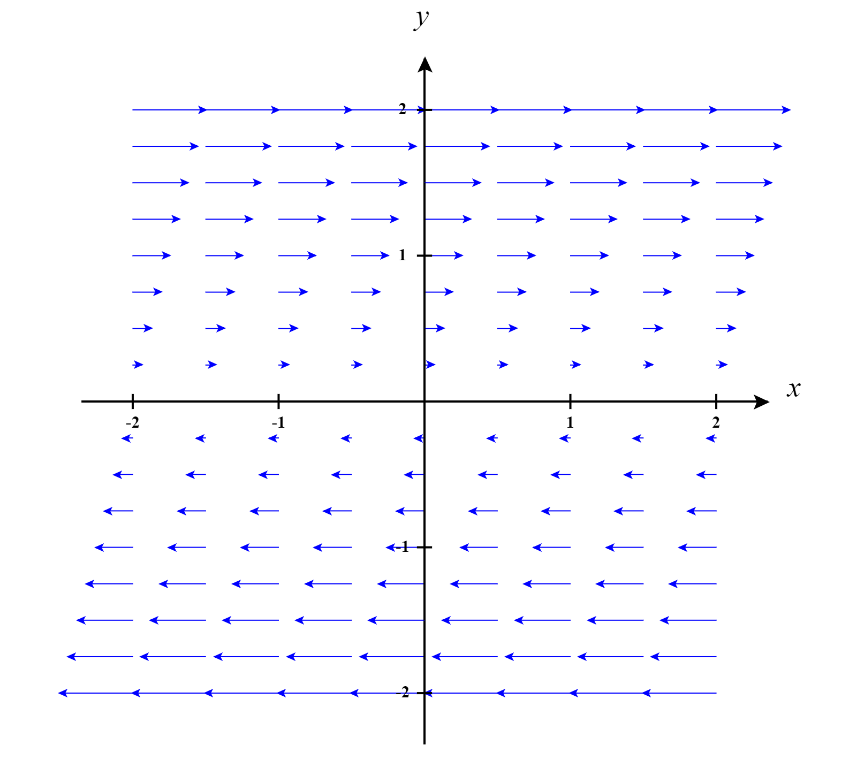
\includegraphics[scale=0.3]{16_3-4pic.png}
	
	\item Compute $\Div \bF$ and $\curl \bF\cdot \bk$ for the vector field $\bF(x,y)=\langle \dfrac{y}{4}, 0 \rangle$, which was plotted above.
	
	%%
	\item Let $C$ be the ellipse 
	\[
	\left( \frac{x}{3} \right)^2 + \left( \frac{y}{4}\right)^2=1.
	\]
	\begin{enumerate}
		\item Parametrize this ellipse to give it a positive orientation.
		
		\item Let $\bF(x,y)=2x \bi + 2y \bj$. Use Green's theorem to find the circulation of $\bF$ around $C$ and its flux across $C$.
	\end{enumerate}  
	\item Let $R$ be the region in the $xy$-plane bounded above by the curve $y=3-x^2$ and below by the curve $y=x^4+1$. Orient this boundary positively. Let 
	\[
	\bF(x,y) = (y+e^x \ln y) \bi + (e^x/y)\bj.
	\]
	Use Green's theorem to find the circulation of $\bF$ around $C$. What happens when you try to use Green's theorem to evaluate the flux of $\bF$ across $C$? Should you use Green's theorem to evaluate the flux integral?
	
	\item Use Green’s Theorem to find the work done by the force $\bF(x,y)=\langle x(x+y),xy^2\rangle$ in moving a particle from the origin along the $x$-axis to $(1,0)$, then along the line segment to $(0,1)$, and then back to the origin along the $y$-axis.
	
	\item \textbf{Looking ahead:} Find a parameterization (a function $\br(s,t)=\langle x(s,t), y(s,t), z(s,t)\rangle$) of the plane through the origin that contains the vectors $\bi-\bj$ and $\bj-\bk$.  Linear algebra ideas may be useful.	
	
\end{enumerate}
}{}

\iftoggle{answers}
{
	\begin{center}{\large \textbf{Math 2551 Worksheet Answers: Curl, Divergence, Green's Theorem}}
	\end{center}

\begin{enumerate}
	
	\item $\nabla\cdot \bF$ is 0 in all quadrants.\\
	$(\nabla \times \bF)\cdot \bk$ is negative in all quadrants.
	
	\item $\nabla\cdot \bF = 0$\\
	$(\nabla \times \bF)\cdot \bk=-\dfrac{1}{4}$. \\
	
	
	\item\begin{enumerate}
		\item $\br(t)=\langle 3 \cos(t), 4\sin(t) \rangle$, $0\leq t \leq 2\pi$.
		
		\item Circulation: 0\\
		Flux: $48\pi$
	\end{enumerate}  
	
	\item Circulation: $-44/15$\\
	Flux: The integrand is very difficult to work with, so we should not use Green's theorem here.
	
	\item $-1/12$
	
	\item One answer (linear algebra!) $\br(s,t)=s\langle 1,-1,0\rangle+t\langle0,1,-1\rangle = \langle s,t-s,-t \rangle$, $s,t\in\R$.
\end{enumerate}
}{}
\iftoggle{solutions}
{
Solutions go here in the same format.
}{}
